\documentclass[10pt]{article}

\usepackage{enumerate}
\usepackage[utf8]{inputenc}
\usepackage[greek, english]{babel}
\usepackage{alphabeta}
\usepackage{libertine}
\usepackage{graphicx}
\usepackage{biblatex}
\usepackage{wrapfig}
\usepackage{hyperref}
\usepackage[table]{xcolor}
\usepackage{mathptmx} % Times New Roman
\usepackage{lipsum}  
\usepackage{makecell}

\pagenumbering{arabic}


\newcommand{\linkstyle}[1]{\color{blue}\underline{#1}}

\graphicspath{ {./resources/} }

\addbibresource{refs.bib}


\title{\Huge A Comprehensive Study on US College Admissions  }

\author{\large Tsirmpas Dimitris\\Athens University of Economics and Business\\Department of Informatics}


\begin{document}
	
	\begin{titlepage}
		\maketitle
		\begin{center}
					
			
\includegraphics[width=1\textwidth]{aueb_logo.jpg}
			
			\large Athens University of Economics and Business
			
			\large Department of Statistics
			
			\large Greece
		\end{center}
	
	\end{titlepage}
	
	\tableofcontents
	\newpage
	
	\section{Abstract}
	US College Admissions have and continue to be a subject of great debate among scholars and analysts. Such educational institutions have an interest in selecting the most qualified applicants using limited data, while the applicants themselves often protest admission requirements, especially those deemed discriminatory in nature. This study aims to analyze the factors that contribute to successful admissions in US colleges and universities by comparing their performance on standardized tests.
	
	
	\section{Introduction}
	The study uses a random sample of 200 students who applied to continue their studies in their respective universities. Their application consisted of three standardized tests testing their skills and knowledge in mathematics, social studies and creative writing. The dataset we used is available at LINK.  An overview of the data contained can be found in Table \ref{tab::dataset}.
	
	We make the assumption that the dataset has been acquired through random, unbiased sampling. We also make the assumption that the records using different IDs represent different students.
	
	The study is structured as follows. In this Section we make general observations about our data and we form our first hypotheses. In Section \ref{sec::results} we follow up with robust analyses and regression models to prove/disprove these hypotheses. Section \ref{sec::conclusions} follows with an overview and discussion about our findings. Finally, in Section \ref{sec::addendum} we include graphs, tables and supporting documents.
	
	\begin{table}
		\centering
		\rowcolors{2}{gray!25}{white}
		\begin{tabular}
			{ |p{1cm} p{1cm} p{5cm} p{3cm}| }
			\hline
			\textbf{Name} & \textbf{Type} & \textbf{Description} & \textbf{Range}\\
			\hline
			Id  & Nominal & The student's ID & [1-200] \\
			Gender  & Binary & The student's gender & \{male, female\} \\
			Race  & Nominal & The student's race & \{white, latin-american, asian, african-american\} \\
			Schtype  & Binary & The type of the student's secondary education institution & \{public, private\} \\
			Prog  & Nominal & The student's previous study cycle  & \{general, vocation, academic \} \\
			Write  & Numeric & The grade on the writing test  & [0-100] \\
			Math  & Numeric & The grade on the mathematics test  & [0-100] \\
			Socst  & Numeric & The grade on the social studies test & [0-100] \\
			\hline
		\end{tabular}
		\caption{An overview of the data used in this study.}
		\label{tab::dataset}
	\end{table}


	The numerical variables contained in the dataset are described in Table \ref{tab::summary_stats}. We observe that they are all almost symmetrical ($-0.5 \leq skew \leq 0.5$), and feature moderate negative (right) skewness with a mean/median hovering just above a score of 50. This indicates most students score around the baseline, most of which pass the exams with a mediocre grade.

	\begin{table}
		\centering
		\rowcolors{2}{gray!25}{white}
		\begin{tabular}
			{ |p{1cm} p{0.5cm} p{0.7cm} p{0.5cm} p{1cm} p{0.7cm} p{0.5cm} p{0.5cm} p{0.5cm} p{0.5cm} p{0.5cm}| }
			\hline
			\textbf{Var.} & \textbf{Obs.} & \textbf{Mean} & \textbf{Std} & \textbf{Median} & \textbf{Trim} & \textbf{Min} & \textbf{Max} & \textbf{Skew} & \textbf{Kurt} & \textbf{SE}\\
			\hline
			Write & $200$ & $52.77$ & $9.48$ & $54$ & $53.36$ & $31$ & $67$ & $-0.47$ & $-0.78$ & $0.67$ \\
			Math & $200$ & $52.65$ & $9.37$ & $52$ & $52.33$ & $33$ & $75$ & $0.28$ & $-0.69$ & $0.66$ \\
			Socst & $200$ & $52.41$ & $10.74$ & $52$ &$ 52.99$ & $26$ & $71$ & $-0.38$ & $-0.57$ & $0.76$ \\
			\hline
		\end{tabular}
		\caption{Summary statistics on the numerical data used in the study.}
		\label{tab::summary_stats}
	\end{table}

	We next study the relationships between the three subjects. As shown in Table \ref{tab::corr}, there is a very statistically significant (p\_value = $0.0000$), positive ($r > 0.5$) relationship between all three subjects. This could be indicative of either one of the variables influencing the other, or an unknown, interfering variable which positively affects the three test scores. We hypothesize the latter, as the existence of such a variable indicating the student's general competence in tests makes intuitive sense. We will refer to this potential, unknown variable as "Competence" in this report.
	
	Since the three subjects are strongly correlated we can explore correlations between the rest of the factors and any of the tests, assuming that a correlation with one strongly indicates with the other two as well. 
	
	We notice a probable correlation between gender and writing scores, as shown in Figure \ref{fig::write_gender}, as well as between the student's program and writing scores, as shown in Figure \ref{fig::write_prog}.
	
	\begin{table}
		\scriptsize
		\centering
		\rowcolors{2}{gray!25}{white}
		\begin{tabular}
			{ |p{1.2cm} | p{1.2cm} p{1.2cm} p{1.2cm} | }
			\hline
			 & \textbf{write} & \textbf{math} & \textbf{socst} \\
			 \hline
			\textbf{write} & \makecell{$1$\\ $0.000$ ****} & - & - \\
			\textbf{math} & \makecell{$0.62$\\ $0.000$ ****} & \makecell{$1$\\ $0.00$ ****} & - \\
			\textbf{socst} & \makecell{$0.60$\\ $0.000$ ****} & \makecell{$0.54$\\ $0.000$**** \\} &\makecell{$1$\\ $0.000$****}\\
			\hline
		\end{tabular}
		\caption{Pearson's correlation coefficient (Holm's correction) between the tests and their p\_values. Stars indicate significance scores: $>1$:'', $0.1$:'*', $0.01$: '**', $0.001$: '***', $<0.0001$: '****'}
		\label{tab::corr}
	\end{table}

	\begin{figure}
		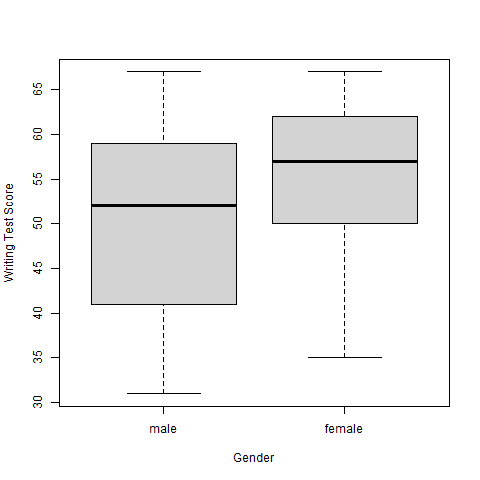
\includegraphics[width=4cm]{write_genre_boxplot.png}
		\centering
		\caption{Boxplot displaying the writing score by gender.}
		\label{fig::write_gender}
	\end{figure}

	\begin{figure}
		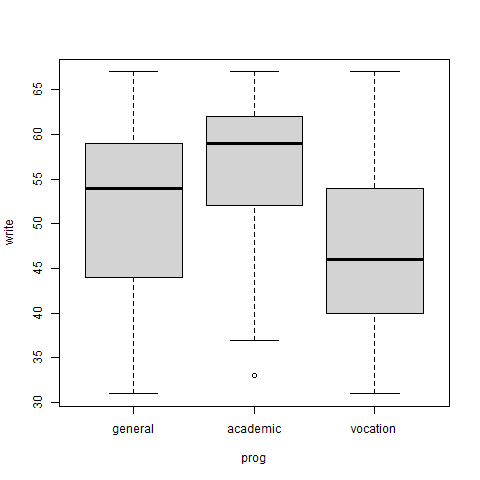
\includegraphics[width=4cm]{write_prog_boxplot.png}
		\centering
		\caption{Boxplot displaying the writing score by current program. Notice the significant differences in means.}
		\label{fig::write_prog}
	\end{figure}
	
	\section{Results}
	\label{sec::results}
	
	\subsection{Writing scores influenced by gender}
	Our exploratory analysis indicated a possible discrepancy between the results of writing tests between men and women, as well as between different programs. We thus investigate whether gender and the candidate's current program play a role in writing test score.
	
	We begin by verifying the preconditions necessary for the standard t-test in order to compare the genders' scores. We compute the mean differences of the samples by subtracting the global mean by the women's scores \parencite{means}, and conclude they are not normal (Shapiro-Wilk normality test, $p\_value = 0.0024$). The variances are not homogeneous (Levene's test $p\_value = 0.0022$), although this should not dissuade us from using a parametric t-test since the relatively large sample size ($N=200$) and balanced groups ($N_{women} = 109, N_{men} = 91$) means the precondition's violation is not significant \parencite{variances}. We will use a parametric test since the distribution of the differences has a normal kurtosis (Jarque-Bera Normality Test \cite{jarque}, $p\_value=0.026$).
	
	We conclude there is a statistically significant difference between the writing scores of men and women (Two-sided Welch Two Sample t-test, $p\_value = 0.0003$) with women having on average 5 more score than men (Welch Two Sample t-test with $H_a = less$, $p\_value = 0.00017$).
	
	
	\subsection{Writing scores influenced by previous program}
	We will now verify the preconditions for the parametric ANOVA test in order to test which programs are correlated with the writing tests' scores. The variances of the residuals are homogeneous (Levene's test $p\_value = 0.0022$), but not normal (Shapiro-Wilk normality test, $p\_value = 0.002$). We will thus use a non-parametric test.
	
	We discover there is a statistically significant difference between the groups (Kruskall-Wallis rank sum test, $p\_value=4e-08$). We can consult the boxplots in Figure \ref{fig::write_prog}, where we observe significant differences between all three groups.
	
	
	\subsection{Building a predictive model}
	Having confirmed our hypotheses regarding the relationships between the various variables and the writing test scores, we attempt to build a model which will predict a candidate's math and social study scores, testing our hypothesis that the three scores are influenced by the same external factors. 
	
	Since there seem to be strong correlations between most independent variables and the writing scores, and since we already established a strong correlation between the scores themselves (attributed to the candidate's \textit{"Competence"}), we will be using a simple, Ordinary Least Squares (OLS) model.
	
	We initially build an OLS model predicting the writing scores which involves all the available variables. This model exhibits a good fit ($R^2_{adj} = 0.4753, F= 37.06 p\_value=2.2e-16, df=194$). We also verify all the preconditions for the regression model; the residuals appear to be normal (Shapiro-Wilk normality test $p\_value = 0.2099$), homogeneous (Levene's Test, $p\_value = 0.1057$) and non-correlated (Durbin-Watson test, $p\_value=0.236$) and there are no significant outliers (see Addendum).
	
	Our current model exhibits high confidence about the gender ($p\_value_{female} = 0.0056$), previous program  ($p\_value_{progacademic} = 0.0025$), writing scores ($p\_value_{write} = 3.57e-08$), social study scores ($p\_value_{socst} = 0.0053$) and the constant ($p\_value_{intercept} = 8.29e-09$). However, it exhibits low confidence about the candidate's race ($p\_value_{raceasian} = 0.05$) and no confidence about his school type ($p\_value=0.6502$). In order to build an optimal model, we consider dropping these two variables. Dropping the candidate's race along with the school type leads to a slight decrease of $R^2_{adj} = 0.4753$. Dropping only the school type on the other hand leads to an improved $R^2_{adj} = 0.4882$. Since the model maintains its confidence about the other variables, we keep this model as the optimal one. A summary of the optimal model can be found in Table \ref{tab::lm_math_peeking}.
	
	We now follow the same procedure for the social studies test. We fit a model involving all available variables, which explains our sample to a decent degree ($R^2_{adj} = 0.4535, F= 17.7 p\_value=2.2e-16, df=188$). We detect an outlier in our precondition verification, a student with an above-average grade in writing but an abysmal one in social studies. Since this individual exerts a significant influence in our model (as it is largely dependent on the writing scores for its predictions) we remove them from the sample. The other preconditions are met, the residuals are sufficiently normal (Shapiro-Wilk normality test $p\_value = 0.0125$), homogeneous (Levene's Test, $p\_value = 0.3394$) and non-correlated (Durbin-Watson test, $p\_value=0.678$).
	
	As mentioned above, this model is reliant on the math and especially on the writing scores, while the rest of the variables are mostly non-statistically significant. We thus employ a stepwise procedure in order to eliminate variables deemed statistically insignificant while retaining, or increasing our models goodness of fit. A summary of the resulting model can be found in Table \ref{tab::lm_socst_peeking}.
	
	
% Table created by stargazer v.5.2.3 by Marek Hlavac, Social Policy Institute. E-mail: marek.hlavac at gmail.com
% Date and time: Sat, May 20, 2023 - 3:44:05 PM
\begin{table}[!htbp] \centering 
  \caption{Linear regression model predicting math test scores, taking into 
          account other test scores.} 
  \label{tab::lm_math_peeking} 
\begin{tabular}{@{\extracolsep{5pt}}lc} 
\\[-1.8ex]\hline 
\hline \\[-1.8ex] 
 & \multicolumn{1}{c}{\textit{Dependent variable:}} \\ 
\cline{2-2} 
\\[-1.8ex] & math \\ 
\hline \\[-1.8ex] 
 genrefemale & $-$2.828$^{***}$ \\ 
  & ($-$4.799, $-$0.858) \\ 
  & \\ 
 progacademic & 3.788$^{***}$ \\ 
  & (1.346, 6.229) \\ 
  & \\ 
 progvocation & $-$0.375 \\ 
  & ($-$3.161, 2.410) \\ 
  & \\ 
 write & 0.404$^{***}$ \\ 
  & (0.266, 0.542) \\ 
  & \\ 
 socst & 0.167$^{***}$ \\ 
  & (0.052, 0.283) \\ 
  & \\ 
 raceasian & 4.978$^{*}$ \\ 
  & ($-$0.017, 9.972) \\ 
  & \\ 
 raceafrican-amer & $-$1.103 \\ 
  & ($-$5.104, 2.898) \\ 
  & \\ 
 racewhite & 2.324 \\ 
  & ($-$0.686, 5.334) \\ 
  & \\ 
 Constant & 20.334$^{***}$ \\ 
  & (13.730, 26.938) \\ 
  & \\ 
\hline \\[-1.8ex] 
Observations & 200 \\ 
R$^{2}$ & 0.509 \\ 
Adjusted R$^{2}$ & 0.488 \\ 
Residual Std. Error & 6.702 (df = 191) \\ 
F Statistic & 24.729$^{***}$ (df = 8; 191) \\ 
\hline 
\hline \\[-1.8ex] 
\textit{Note:}  & \multicolumn{1}{r}{$^{*}$p$<$0.1; $^{**}$p$<$0.05; $^{***}$p$<$0.01} \\ 
\end{tabular} 
\end{table} 

	
% Table created by stargazer v.5.2.3 by Marek Hlavac, Social Policy Institute. E-mail: marek.hlavac at gmail.com
% Date and time: Sat, May 27, 2023 - 7:11:52 PM
\begin{table}[!htbp] \centering 
  \caption{Linear regression model predicting social study test scores, taking into 
          account other test scores.} 
  \label{tab::lm_socst_peeking} 
\begin{tabular}{@{\extracolsep{5pt}}lc} 
\\[-1.8ex]\hline 
\hline \\[-1.8ex] 
 & \multicolumn{1}{c}{\textit{Dependent variable:}} \\ 
\cline{2-2} 
\\[-1.8ex] & socst \\ 
\hline \\[-1.8ex] 
 progacademic & 2.276 \\ 
  & p = 0.137 \\ 
  & \\ 
 progvocation & $-$2.669 \\ 
  & p = 0.118 \\ 
  & \\ 
 write & 0.446$^{***}$ \\ 
  & p = 0.00000 \\ 
  & \\ 
 math & 0.242$^{***}$ \\ 
  & p = 0.004 \\ 
  & \\ 
 Constant & 15.610$^{***}$ \\ 
  & p = 0.0003 \\ 
  & \\ 
\hline \\[-1.8ex] 
Observations & 200 \\ 
R$^{2}$ & 0.441 \\ 
Adjusted R$^{2}$ & 0.429 \\ 
Residual Std. Error & 8.111 (df = 195) \\ 
F Statistic & 38.416$^{***}$ (df = 4; 195) \\ 
\hline 
\hline \\[-1.8ex] 
\textit{Note:}  & \multicolumn{1}{r}{$^{*}$p$<$0.1; $^{**}$p$<$0.05; $^{***}$p$<$0.01} \\ 
\end{tabular} 
\end{table} 


	
	\section{Conclusions \& Discussion}
	\label{sec::conclusions}
	\lipsum[23-28]
	
	\section{Bibliography}
	\printbibliography
	
	\section{Addendum}
	\label{sec::addendum}
	\lipsum[31-35]
	
\end{document}